\section{Introduction}

In this student project, a wireless communication system is implemented in the GNU Radio framework.  GNU Radio is a development toolkit that provides signal processing blocks for software-defined radios and signal processing systems. These blocks are connected in flowgraphs, which can be built visually in the GNU Radio Companion or by coding in Python. An example of a wireless communication chain is given in \reff{commchain_intro}.


\begin{figure}[H]
    \centering
    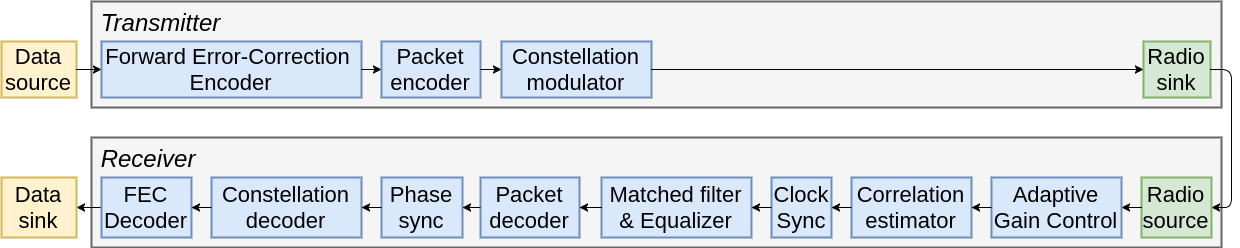
\includegraphics[width=1\textwidth]{img_commchain/overview.png}
    \caption{Communication chain}
    \label{fig:commchain_intro}
\end{figure}

We developed several new blocks to integrate functionality currently not possible in GNU Radio. They will be discussed throughout the report. Extra attention is paid to the packet encoder and decoder in the communication chain. A packet encoder encapsulates the incoming stream into packets, consisting of a preamble, header (containing packet length), payload and checksum. In particular, a flexible packet encoder is implemented, supporting different constellations for preamble, header and payload. The new packet encoder/decoder pair also supports soft-decision error correction and varying packet lengths.\medskip

A small introduction to GNU Radio is provided. The first part of the report focuses on the packet encoder/decoder. The existing packet encoder/decoder pair is evaluated and new, improved blocks are implemented. The second part integrates the new packet encoder/decoder pair in a full-featured wireless communication chain. Problems with the existing frame synchronizer are examined and the improved implementation is discussed. At the end of the report, GNU Radio challenges and limitations are discussed as well as some lessons learned. \medskip

The examples and developed blocks are combined in a GNU Radio module called \textit{packetizer}, located at \url{https://tclgit.epfl.ch/semester-projects/17S-Verelst-GNURadio}.

